
\subsection{算子 $\mathfrak r$ 的代数表述 I：
$\operatorname{Der}B(C_1,C_0;D)$ 及其同伦不变性}
\label{subsec:7-4-7}
\liftIndex{I292}

下一小节将用 $L_\infty$ 代数的语言
重新表述定理~\ref{thm:3-8-71}，
并陈述算子 $\mathfrak r$ 的主要性质。
为此，先准备一些代数材料。

设 $C_1,C_0$ 为滤过 $A_\infty$ 代数，
$D$ 为 $(C_1,C_0)$-滤过 $A_\infty$ 双模。
置
\begin{equation}
BDB=
\widehat B(C_1[1])\widehat\otimes
D[1]\widehat\otimes
\widehat B(C_0[1]).
\tag{7.4.138}\label{eq:7-4-138}
\end{equation}
$BDB$ 是
$\widehat B(C_1[1])$--$\widehat B(C_0[1])$
上的双余模。
也就是说，存在滤过同态
\begin{equation}
\left\{
\begin{aligned}
\Delta_{\mathrm{Right}}\colon
BDB&\longrightarrow
BDB\widehat\otimes\widehat B(C_0[1]),\\
\Delta_{\mathrm{Left}}\colon
BDB&\longrightarrow
\widehat B(C_1[1])\widehat\otimes BDB,
\end{aligned}
\right.
\tag{7.4.139}\label{eq:7-4-139}
\end{equation}
满足
\begin{equation}
\left\{
\begin{aligned}
\Delta_{\mathrm{Right}}\circ\Delta_{\mathrm{Left}}
&=\Delta_{\mathrm{Left}}\circ\Delta_{\mathrm{Right}},\\
(1\widehat\otimes\Delta_{\mathrm{Left}})
\circ\Delta_{\mathrm{Left}}
&=(\Delta\widehat\otimes1)
\circ\Delta_{\mathrm{Left}},\\
(\Delta_{\mathrm{Right}}\widehat\otimes1)
\circ\Delta_{\mathrm{Right}}
&=(1\widehat\otimes\Delta)
\circ\Delta_{\mathrm{Right}}.
\end{aligned}
\right.
\tag{7.4.140}\label{eq:7-4-140}
\end{equation}

若滤过同态
$\widehat\psi\colon BDB\to BDB$
满足
\[
\begin{aligned}
\Delta_{\mathrm{Left}}\circ\widehat\psi
&=(1\widehat\otimes\widehat\psi)
\circ\Delta_{\mathrm{Left}},\\
\Delta_{\mathrm{Right}}\circ\widehat\psi
&=(\widehat\psi\widehat\otimes1)
\circ\Delta_{\mathrm{Right}},
\end{aligned}
\]
则称它为\emph{双余导子}。
以 $\operatorname{Der}B_0(D[1])$
表示所有双余导子 $\widehat\psi$ 所成的集合。

$D$ 上的滤过 $A_\infty$ 双模结构
由式~\eqref{eq:3-7-2}
在 $BDB$ 上确定一个微分 $\widehat d$。
注意，$\widehat d$ 不是双余导子；事实上
\[
\Delta_{\mathrm{Left}}\circ\widehat d
=
(\widehat d\widehat\otimes1
+1\widehat\otimes\widehat d)
\circ\Delta_{\mathrm{Left}}.
\]
定义
\begin{equation}
\delta(\widehat\psi)
=\widehat d\circ\widehat\psi
-(-1)^{\deg\widehat\psi}
\widehat\psi\circ\widehat d.
\tag{7.4.141.1}\label{eq:7-4-141-1}
\end{equation}
容易验证，
$\delta(\widehat\psi)$ 是双余导子
\translatornote{源书这里只称其为 coderivation；但当前空间由同时保持左右余作用的 bicoderivation 构成，且 $\delta$ 要在 $\operatorname{Der}B_0(D[1])$ 上定义微分。译稿据此明确写作“双余导子”。见疑误 A-0595。}。
再定义
\begin{equation}
[\widehat\psi^1,\widehat\psi^2]
=-\frac12\left(
\widehat\psi^1\circ\widehat\psi^2
-(-1)^{\deg\widehat\psi^1\deg\widehat\psi^2}
\widehat\psi^2\circ\widehat\psi^1
\right).
\tag{7.4.141.2}\label{eq:7-4-141-2}
\end{equation}
于是
\[
\bigl(\operatorname{Der}B_0(D[1]),
\delta,[\ ,\ ]\bigr)
\]
成为微分分次李代数。

可以把 $\operatorname{Der}B_0(D[1])$
等同于
\[
\begin{aligned}
CH(D[1],D[1])
=\prod_{k_1,k_0\in\mathbb Z_{\ge0}}
\operatorname{Hom}^{\mathrm{filt}}\Bigl(
&\widehat B_{k_1}(C_1[1])
\widehat\otimes D[1]\\
&\widehat\otimes
\widehat B_{k_0}(C_0[1]),D[1]\Bigr),
\end{aligned}
\]
具体如下。
设
\[
(\psi_{k_1,k_0})_{k_1,k_0\in\mathbb Z_{\ge0}}
\in CH(D[1],D[1]).
\]
置
\[
\begin{aligned}
&\widehat\psi(\mathbf x\otimes y\otimes\mathbf z)\\
&\quad=
\sum_{c_1,c_2}
(-1)^{
\deg\psi\,
\deg'\mathbf x_{c_1}^{(2;1)}}
\mathbf x_{c_1}^{(2;1)}
\otimes
\psi\bigl(
\mathbf x_{c_1}^{(2;2)}
\otimes y\otimes
\mathbf z_{c_2}^{(2;1)}
\bigr)
\otimes
\mathbf z_{c_2}^{(2;2)}.
\end{aligned}
\]
容易看出，
\[
(\psi_{k_1,k_0})_{k_1,k_0\in\mathbb Z_{\ge0}}
\longmapsto\widehat\psi
\]
诱导同构
\begin{equation}
CH(D[1],D[1])
\cong\operatorname{Der}B_0(D[1]).
\tag{7.4.142}\label{eq:7-4-142}
\end{equation}

定义
\[
CH^{\mathrm{unit}}(D[1],D[1])
\cong
\operatorname{Der}B^{\mathrm{unit}}_0(D[1])
\]
为 $\operatorname{Der}B_0(D[1])$ 中
满足下式的所有元素 $\varphi$ 所成集合：
\[
\begin{aligned}
\varphi\bigl(
(\mathbf x_1\otimes\mathbf e\otimes\mathbf x_2)
\otimes y\otimes\mathbf z
\bigr)
&=0,\\
\varphi\bigl(
\mathbf x\otimes y\otimes
(\mathbf z_1\otimes\mathbf e\otimes\mathbf z_2)
\bigr)
&=0.
\end{aligned}
\]

有如下两个等式：
\begin{equation}
\begin{aligned}
&(\delta\widehat\psi)_{k_1,k_0}
(\mathbf x\otimes y\otimes\mathbf z)\\
&=
\sum_{c_1,c_2}
(-1)^{\deg\psi\,
\deg'\mathbf x_{c_1}^{(2;1)}}
\mathfrak n\Bigl(
\mathbf x_{c_1}^{(2;1)}
\otimes
\psi(\mathbf x_{c_1}^{(2;2)}
\otimes y\otimes\mathbf z_{c_2}^{(2;1)})
\otimes\mathbf z_{c_2}^{(2;2)}
\Bigr)\\
&\quad+
\sum_{c_1,c_2}
(-1)^{\deg\psi+
\deg'\mathbf x_{c_1}^{(2;1)}+1}
\psi\Bigl(
\mathbf x_{c_1}^{(2;1)}
\otimes
\mathfrak n(\mathbf x_{c_1}^{(2;2)}
\otimes y\otimes\mathbf z_{c_2}^{(2;1)})
\otimes\mathbf z_{c_2}^{(2;2)}
\Bigr)\\
&\quad-
\psi(\widehat d(\mathbf x),y,\mathbf z)
-(-1)^{\deg'\mathbf x+\deg' y}
\psi(\mathbf x,y,\widehat d(\mathbf z)).
\end{aligned}
\tag{7.4.143}\label{eq:7-4-143}
\end{equation}
\begin{equation}
\begin{aligned}
&[\psi^1,\psi^2]_{k_1,k_0}
(\mathbf x\otimes y\otimes\mathbf z)\\
&=
\frac12\sum_{c_1,c_2}
(-1)^{\deg\psi^2\,
\deg'\mathbf x_{c_1}^{(2;1)}+1}
\psi^1\Bigl(
\begin{aligned}
&\mathbf x_{c_1}^{(2;1)}
\otimes
\psi^2(\mathbf x_{c_1}^{(2;2)}
\otimes y\otimes\mathbf z_{c_2}^{(2;1)})\\[-.2em]
&\qquad{}\otimes\mathbf z_{c_2}^{(2;2)}
\end{aligned}
\Bigr)\\
&\quad+
\frac12\sum_{c_1,c_2}
(-1)^{\deg\psi^1(
\deg'\mathbf x_{c_1}^{(2;1)}+\deg\psi^2)}
\psi^2\Bigl(
\begin{aligned}
&\mathbf x_{c_1}^{(2;1)}
\otimes
\psi^1(\mathbf x_{c_1}^{(2;2)}
\otimes y\otimes\mathbf z_{c_2}^{(2;1)})\\[-.2em]
&\qquad{}\otimes\mathbf z_{c_2}^{(2;2)}
\end{aligned}
\Bigr).
\end{aligned}
\tag{7.4.144}\label{eq:7-4-144}
\end{equation}
这里左端是 $CH(D[1],D[1])$ 中
与
\[
[\widehat\psi^1,\widehat\psi^2]
\in\operatorname{Der}B_0(D[1])
\]
对应的元素
\translatornote{源书此处写 $\operatorname{Der}B(D[1])$；但该空间到下一条定义--命题才引入，而这里两个输入及其括号都属于已经构成微分分次李代数的理想 $\operatorname{Der}B_0(D[1])$。见疑误 A-0596。}。

\begin{statement}{命题--定义}{7.4.145}
\label{defprop:7-4-145}\itshape
存在一个记作
$\operatorname{Der}B(D[1])$
的微分分次李代数，
它以 $\operatorname{Der}B_0(D[1])$ 为理想，
并且存在微分分次李代数的正合列
\begin{equation}
0\longrightarrow
\operatorname{Der}B_0(D[1])
\longrightarrow
\operatorname{Der}B(D[1])
\longrightarrow
\operatorname{Der}B(C_1[1])
\oplus\operatorname{Der}B(C_0[1])
\longrightarrow0.
\tag{7.4.146}\label{eq:7-4-146}
\end{equation}
$\operatorname{Der}B^{\mathrm{unit}}_0(D[1])$
也有类似结论。
\end{statement}

\begin{remark}{7.4.147}\label{rem:7-4-147}
借助滤过 $A_\infty$ 范畴的概念
\liftIndex{I293}（见\textbf{[Fuk02II]}），
可以如下重新解释命题--定义~\ref{defprop:7-4-145}。
考虑含两个对象 $c_1,c_0$ 的滤过
$A_\infty$ 范畴 $\mathcal C$，
其态射为
\[
\mathcal C(c_1,c_1)=C_1,\qquad
\mathcal C(c_0,c_0)=C_0,\qquad
\mathcal C(c_1,c_0)=D,\qquad
\mathcal C(c_0,c_1)=0.
\]
这是\textbf{[Sei06]}意义下的一种
有向 $A_\infty$ 范畴，
只不过它不满足
$\mathcal C(c_i,c_i)=\mathbb Q$。
按定义，$\mathcal C$ 的 Hochschild 复形
是直和复形
\[
\operatorname{Der}B(C_1[1])
\oplus\operatorname{Der}B_0(D[1])
\oplus\operatorname{Der}B(C_0[1]).
\]
Hochschild 复形可与恒等函子到自身的
预自然变换所成复形等同；
见\textbf{[Fuk97II, Fuk02II]}。
由滤过 $A_\infty$ 范畴的一般结果，
它具有微分分次李代数结构，
而这正是 $\operatorname{Der}B(D[1])$。
\end{remark}

\begin{proof}[命题--定义~\ref{defprop:7-4-145} 的证明]
置
\begin{equation}
\operatorname{Der}B(D[1])
=
\operatorname{Der}B(C_1[1])
\oplus\operatorname{Der}B_0(D[1])
\oplus\operatorname{Der}B(C_0[1]).
\tag{7.4.148}\label{eq:7-4-148}
\end{equation}
其上的上边界算子 $\delta$
已经由式~\eqref{eq:7-4-143}
及两端代数上的同一构造定义。
设
\[
\begin{aligned}
\varphi^i
&=(\varphi^i_k)_{k\in\mathbb Z_{\ge0}}
\in CH(C_i[1],C_i[1])
\cong\operatorname{Der}B(C_i[1]),\\
\psi
&=(\psi_{k_1,k_0})_{k_1,k_0\in\mathbb Z_{\ge0}}
\in CH(D[1],D[1])
\cong\operatorname{Der}B_0(D[1]).
\end{aligned}
\]
定义
\[
\begin{aligned}
&[\varphi^1,\psi]_{k_1,k_0}
(\mathbf x\otimes y\otimes\mathbf z)\\
&\quad=
\frac12\sum_c
(-1)^{\deg\varphi^1(
\deg'\mathbf x_c^{(3;1)}+\deg\psi)}
\psi\bigl(
\mathbf x_c^{(3;1)}
\otimes\varphi^1(\mathbf x_c^{(3;2)})
\otimes\mathbf x_c^{(3;3)}
\otimes y\otimes\mathbf z
\bigr),\\[.4em]
&[\psi,\varphi^0]_{k_1,k_0}
(\mathbf x\otimes y\otimes\mathbf z)\\
&\quad=
\frac12\sum_c
(-1)^{\deg\varphi^0(
\deg'\mathbf x+\deg' y+
\deg'\mathbf z_c^{(3;1)})+1}
\psi\bigl(
\begin{aligned}
&\mathbf x\otimes y\otimes
\mathbf z_c^{(3;1)}\\[-.2em]
&\qquad{}\otimes\varphi^0(\mathbf z_c^{(3;2)})
\otimes\mathbf z_c^{(3;3)}
\end{aligned}
\bigr),\\
&[\varphi^1,\varphi^0]=0.
\end{aligned}
\]
直接验证即可看出，这些运算具有所需性质。
\end{proof}

从注~\ref{rem:7-4-147}
所述滤过 $A_\infty$ 范畴的观点看，
除上述括号外的其他括号都为零，
这是 $\mathcal C(c_0,c_1)=0$ 的推论。

\begin{theorem}{7.4.149}\label{thm:7-4-149}
设 $C_i$ 与 $C'_i$ 有隙地同伦等价
（$i=0,1$）。
设 $D$ 是
$(C_1,\mathfrak m)$、$(C_0,\mathfrak m)$
上的有隙滤过 $A_\infty$ 双模，
$D'$ 是
$(C'_1,\mathfrak m)$、$(C'_0,\mathfrak m)$
上的这种双模。
假设在从 $C_i$ 到 $C'_i$ 的同伦等价之上，
$D$ 与 $D'$ 有隙地同伦等价。
则存在滤过 $L_\infty$ 代数之间严格、有隙且滤过的
同伦等价
\[
\operatorname{Der}B(D[1])
\longrightarrow
\operatorname{Der}B(D'[1]),
\]
使它与定理~\ref{thm:7-4-41}
得到的同伦等价共同组成下列交换图式：

\par\medskip\noindent\begin{minipage}{\textwidth}
\centering
\resizebox{.86\textwidth}{!}{$\displaystyle
\begin{array}{ccc}
\operatorname{Der}B(D[1])
&\longrightarrow&
\operatorname{Der}B(C_1[1])
\oplus\operatorname{Der}B(C_0[1])
\\[-.1em]
\Big\downarrow&&\Big\downarrow
\\[-.1em]
\operatorname{Der}B(D'[1])
&\longrightarrow&
\operatorname{Der}B(C'_1[1])
\oplus\operatorname{Der}B(C'_0[1]).
\end{array}$}
\par\smallskip
{\renewcommand{\thefigure}{7.4.4}\refstepcounter{figure}
\normalfont\bfseries 图式~\thefigure\label{diag:7-4-4}}
\end{minipage}\par\medskip
\end{theorem}

\begin{proof}
只须证明 $C'_i$ 与 $D'$
分别为 $C_i$ 与 $D$ 的典范模型的情形。
置 $C'_i=H_i$、$D'=H$。
分别为 $D,C_i$ 取调和投影
$\Pi_H,\Pi_{H_i}$ 以及格林算子
$\mathfrak G,\mathfrak G_i$。
我们将把 $C_i$ 的算子
$\mathfrak g^{(i)}$
（它们已在定理~\ref{thm:7-4-41} 的证明中定义）
与下列算子一同构造：
\begin{equation}
\begin{aligned}
\mathfrak g_{\ell_1,\ell,\ell_0}\colon&
E_{\ell_1}\bigl(\operatorname{Der}B(C_1[1])[1]\bigr)
\otimes
E_\ell\bigl(\operatorname{Der}B_0(D[1])[1]\bigr)\\
&\otimes
E_{\ell_0}\bigl(\operatorname{Der}B(C_0[1])[1]\bigr)
\longrightarrow
\operatorname{Der}B_0(H[1]).
\end{aligned}
\tag{7.4.150}\label{eq:7-4-150}
\end{equation}
这些算子将定义所需的滤过同伦等价
\[
\operatorname{Der}B(D[1])
\longrightarrow
\operatorname{Der}B(H[1]).
\]

按定义，
$\mathfrak g_{\ell_1,\ell,\ell_0}$
由算子族
\begin{equation}
\begin{aligned}
&\mathfrak g_{\ell_1,\ell,\ell_0;k_1,k_0}\colon
E_{\ell_1}\bigl(\operatorname{Der}B(C_1[1])[1]\bigr)
\otimes
E_\ell\bigl(\operatorname{Der}B_0(D[1])[1]\bigr)\\
&\quad\otimes
E_{\ell_0}\bigl(\operatorname{Der}B(C_0[1])[1]\bigr)
\otimes B_{k_1}(H_1[1])
\otimes H[1]\otimes B_{k_0}(H_0[1])
\longrightarrow H[1]
\end{aligned}
\tag{7.4.151.1}\label{eq:7-4-151-1}
\end{equation}
诱导。
我们仿照定理~\ref{thm:7-4-41} 的证明，
把它与下列算子一同定义：
\begin{equation}
\begin{aligned}
&\mathfrak f_{\ell_1,\ell,\ell_0;k_1,k_0}\colon
E_{\ell_1}\bigl(\operatorname{Der}B(C_1[1])[1]\bigr)
\otimes
E_\ell\bigl(\operatorname{Der}B_0(D[1])[1]\bigr)\\
&\quad\otimes
E_{\ell_0}\bigl(\operatorname{Der}B(C_0[1])[1]\bigr)
\otimes B_{k_1}(H_1[1])
\otimes H[1]\otimes B_{k_0}(H_0[1])
\longrightarrow D[1].
\end{aligned}
\tag{7.4.151.2}\label{eq:7-4-151-2}
\end{equation}

以 $G(k,\mathbf Y;C_i)$ 表示
定理~\ref{thm:7-4-41} 的证明中定义的
带附加结构的平面树集合。
记号中写出 $C_i$，
是为了说明论证究竟应用于 $C_1$ 还是 $C_0$。
设
\[
\begin{aligned}
\mathbf Y^i
&=(Y^i_1,\ldots,Y^i_{\ell_i}),
&Y^i_j&\in
\operatorname{Der}B(\overline C_i[1]),\\
\mathbf Y
&=(Y_1,\ldots,Y_\ell),
&Y_j&\in
\operatorname{Der}B_0(\overline D[1]).
\end{aligned}
\]
这里把中间输入写作
$Y_j\in\operatorname{Der}B_0(\overline D[1])$
\translatornote{源书写 $Y_j\in\operatorname{Der}B_0(\overline H[1])$；但它是式 (7.4.150)--(7.4.151.1) 中从 $D$ 转移到 $H$ 的输入，且下文 $Y(v)$ 的源、靶均以 $\overline D$ 为中间模。见疑误 A-0597。}。
考虑一棵带附加结构的平面树
\[
\Gamma=
\bigl(
|\Gamma|;
\mathbf Y^1(\,\cdot\,),
\mathbf Y(\,\cdot\,),
\mathbf Y^0(\,\cdot\,);
\beta(\,\cdot\,)
\bigr),
\]
要求它满足：

\begin{enumerate}
\item[\textup{(7.4.152.1)}]\label{cond:7-4-152-1}
$\Gamma$ 含有一个子图 $\Gamma_0$，
它同构于区间 $[0,1]$ 的一个单纯剖分。
以 $v_0$ 表示对应于 $0\in[0,1]$ 的顶点，
以 $v_{\mathrm{first}}$ 表示对应于
$1\in[0,1]$ 的顶点。
这两个顶点称为外顶点，
$\Gamma_0$ 的其余顶点都称为内顶点。

\item[\textup{(7.4.152.2)}]\label{cond:7-4-152-2}
$|\Gamma|\setminus|\Gamma_0|$ 的闭包分解为
\[
\bigcup_{j=1}^{a_1}|\Gamma^1_j|
\ \cup\
\bigcup_{j=1}^{a_0}|\Gamma^0_j|.
\]
把 $v_0$ 放在上方、
$v_{\mathrm{first}}$ 放在下方时，
$|\Gamma^1_j|$ 位于 $\Gamma_0$ 左侧，
$|\Gamma^0_j|$ 位于 $\Gamma_0$ 右侧。

\item[\textup{(7.4.152.3)}]\label{cond:7-4-152-3}
给 $|\Gamma^i_j|$ 配置
$\mathbf Y^i$ 与 $\beta$ 的限制，
所得树记为 $\Gamma^i_j$。
则
\[
\Gamma^i_j\in
G(k^i_j,\mathbf Y^i_j;C_i),
\qquad
\sum_jk^i_j=k_i.
\]
并且
\[
\mathbf Y^i=\bigsqcup_j\mathbf Y^i_j,
\]
其中右端是不交并。

\item[\textup{(7.4.152.4)}]\label{cond:7-4-152-4}
交集
$|\Gamma^i_j|\cap|\Gamma_0|$
恰含一个点；
该点同时等同于 $\Gamma^i_j$ 的第 $0$ 个顶点
和 $\Gamma_0$ 的一个内顶点。

\item[\textup{(7.4.152.5)}]\label{cond:7-4-152-5}
$\Gamma_0$ 的每个内顶点 $v$
都是 $N$ 型或 $Y$ 型。
对每个 $N$ 型顶点 $v$，
指定 $\beta(v)\in G$。
若 $\beta(v)=\beta_0=0$，
则 $v$ 至少邻接三条边。

对每个 $Y$ 型顶点 $v$，
指定 $Y(v)\in\mathbf Y$。
分别以
$C^0_Y(\Gamma_0)$、
$C^0_N(\Gamma_0)$
表示全体 $Y$ 型、$N$ 型顶点。
映射 $v\mapsto Y(v)$
给出 $C^0_Y(\Gamma_0)$ 与
$\mathbf Y$ 之间的双射。
若 $Y$ 型顶点 $v$ 邻接
$k^1_v+k^0_v+1$ 条边，
其中 $k^1_v$ 条位于 $\Gamma_0$ 左侧，
$k^0_v$ 条位于 $\Gamma_0$ 右侧，
另有一条边属于 $\Gamma_0$，
则
\[
Y(v)\in
\operatorname{Hom}\Bigl(
B_{k^1_v}(\overline C_1[1])
\otimes\overline D[1]\otimes
B_{k^0_v}(\overline C_0[1]),
\overline D[1]\Bigr).
\]
\end{enumerate}

\par\medskip\noindent\begin{minipage}{\textwidth}
\centering
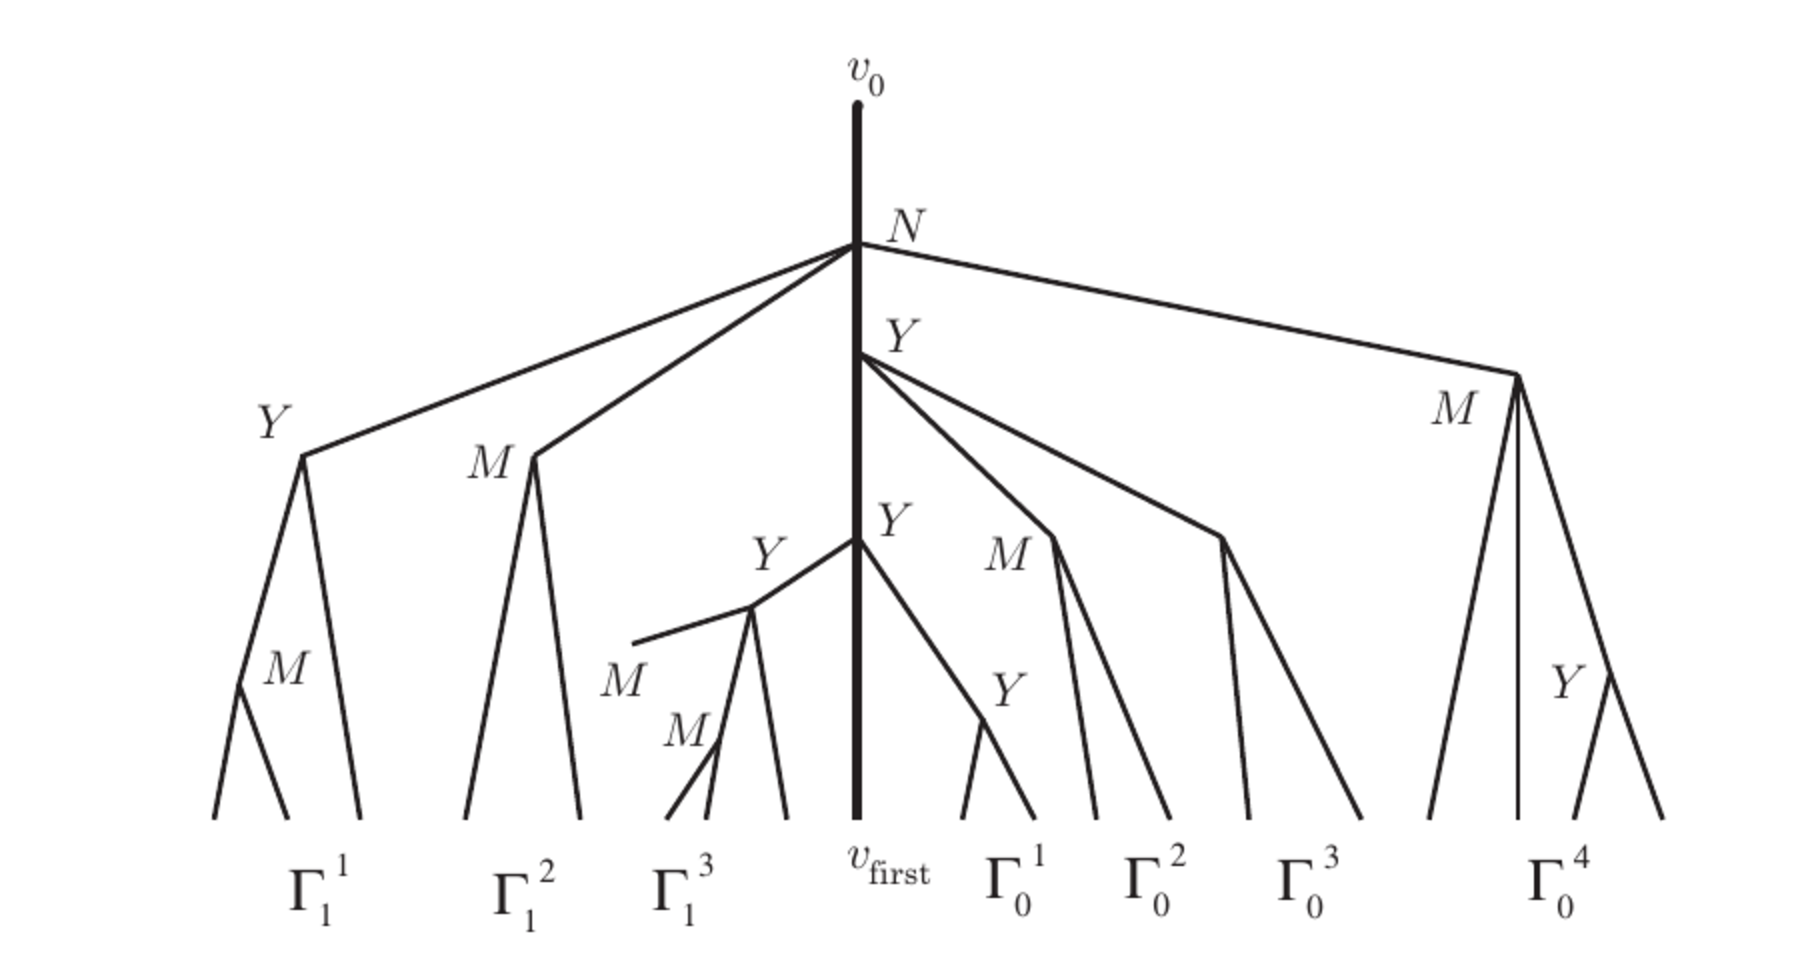
\includegraphics[width=.78\textwidth]{chapters/ch07-transversality/figures/phys-644-figure-7-4-16-clean-crop.png}
\par\smallskip
{\renewcommand{\thefigure}{7.4.16}\refstepcounter{figure}
\normalfont\bfseries 图~\thefigure\label{fig:7-4-16}}
\end{minipage}\par\medskip

以
$G(k_1,k_0;\mathbf Y^1,\mathbf Y,\mathbf Y^0)$
表示满足条件
\textup{(7.4.152.1)--(7.4.152.5)}
的所有 $\Gamma$ 所成集合
\translatornote{源书此处误写“满足 (7.4.136)”；该编号属于前一小节的一则注，当前树的条件是紧前的 (7.4.152.1)--(7.4.152.5)。见疑误 A-0598。}。
置
\[
\beta(\Gamma)=\sum_v\beta(v),
\qquad
E(\Gamma)=E(\beta(\Gamma)),
\qquad
\mu(\Gamma)=\mu(\beta(\Gamma)).
\]
下面定义
\[
\begin{aligned}
\mathfrak g(\Gamma)\colon&
B_{k_1}(\overline H_1[1])
\otimes\overline H[1]\otimes
B_{k_0}(\overline H_0[1])
\longrightarrow\overline H[1],\\
\mathfrak f(\Gamma)\colon&
B_{k_1}(\overline H_1[1])
\otimes\overline H[1]\otimes
B_{k_0}(\overline H_0[1])
\longrightarrow\overline D[1].
\end{aligned}
\]
按 $\Gamma_0$ 的内顶点数归纳定义。
若 $\Gamma_0$ 没有内顶点，
则 $k_1=k_0=0$，并置
\[
\mathfrak f(\Gamma)=\operatorname{id},
\qquad
\mathfrak g(\Gamma)=0.
\]

现在假设 $\Gamma_0$ 至少有一个内顶点。
设 $e_0$ 是以 $v_0$ 为端点的边，
并置 $\partial e_0=\{v_0,v_1\}$。
注意 $v_1$ 必为内顶点。
可以重新编号
$\Gamma^i_j$（$j=1,\ldots,a_i$），
使得
\[
\Gamma\setminus(e_0\cup v_0\cup v_1)
=
\bigcup_{j=1}^{b_1}\Gamma^1_j
\ \cup\ \Gamma'_0\ \cup\
\bigcup_{j=1}^{b_0}\Gamma^0_j,
\]
并使
\[
\Gamma^1_1,\Gamma^1_2,\ldots,\Gamma^1_{b_1},
\Gamma'_0,
\Gamma^0_1,\ldots,\Gamma^0_{b_0}
\]
按平面的逆时针定向所诱导的循环次序排列。

\par\medskip\noindent\begin{minipage}{\textwidth}
\centering
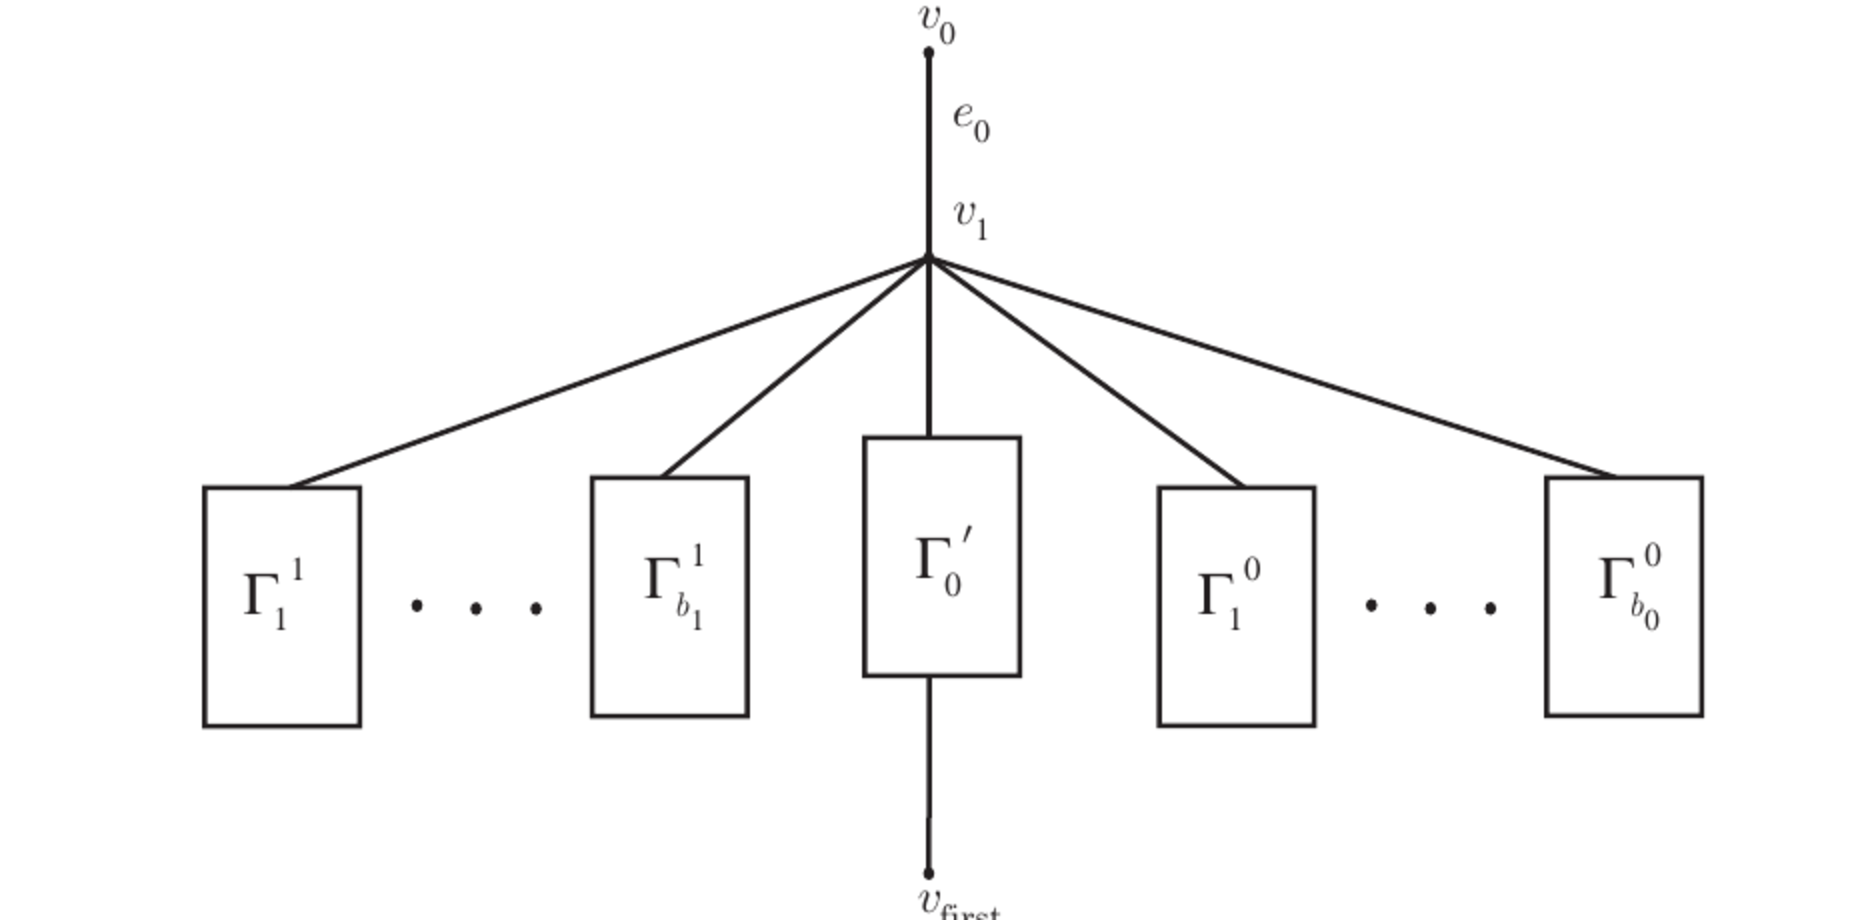
\includegraphics[width=.72\textwidth]{chapters/ch07-transversality/figures/phys-645-figure-7-4-17-final-crop.png}
\par\smallskip
{\renewcommand{\thefigure}{7.4.17}\refstepcounter{figure}
\normalfont\bfseries 图~\thefigure\label{fig:7-4-17}}
\end{minipage}\par\medskip

若 $v_1$ 为 $N$ 型，置
\[
\begin{aligned}
\mathfrak f(\Gamma)
={}&
\mathfrak G\circ\mathfrak n_{b_1,b_0;\beta}
\circ\Bigl(
\mathfrak f^{(1)}(\Gamma^1_1)
\widehat\otimes'\cdots\widehat\otimes'
\mathfrak f^{(1)}(\Gamma^1_{b_1})
\widehat\otimes'\mathfrak f(\Gamma'_0)\\
&\hspace{37mm}{}
\widehat\otimes'\mathfrak f^{(0)}(\Gamma^0_1)
\widehat\otimes'\cdots\widehat\otimes'
\mathfrak f^{(0)}(\Gamma^0_{b_0})
\Bigr),\\
\mathfrak g(\Gamma)
={}&
\Pi_H\circ\mathfrak n_{b_1,b_0;\beta}
\circ\Bigl(
\mathfrak f^{(1)}(\Gamma^1_1)
\widehat\otimes'\cdots\widehat\otimes'
\mathfrak f^{(1)}(\Gamma^1_{b_1})
\widehat\otimes'\mathfrak f(\Gamma'_0)\\
&\hspace{37mm}{}
\widehat\otimes'\mathfrak f^{(0)}(\Gamma^0_1)
\widehat\otimes'\cdots\widehat\otimes'
\mathfrak f^{(0)}(\Gamma^0_{b_0})
\Bigr).
\end{aligned}
\]
$\widehat\otimes'$ 的定义见式~\eqref{eq:7-4-53}。

若 $v_1$ 为 $Y$ 型，置
\[
\begin{aligned}
\mathfrak f(\Gamma)
={}&
\mathfrak G\circ Y(v_1)
\circ\Bigl(
\mathfrak f^{(1)}(\Gamma^1_1)
\widehat\otimes'\cdots\widehat\otimes'
\mathfrak f^{(1)}(\Gamma^1_{b_1})
\widehat\otimes'\mathfrak f(\Gamma'_0)\\
&\hspace{37mm}{}
\widehat\otimes'\mathfrak f^{(0)}(\Gamma^0_1)
\widehat\otimes'\cdots\widehat\otimes'
\mathfrak f^{(0)}(\Gamma^0_{b_0})
\Bigr),\\
\mathfrak g(\Gamma)
={}&
\Pi_H\circ Y(v_1)
\circ\Bigl(
\mathfrak f^{(1)}(\Gamma^1_1)
\widehat\otimes'\cdots\widehat\otimes'
\mathfrak f^{(1)}(\Gamma^1_{b_1})
\widehat\otimes'\mathfrak f(\Gamma'_0)\\
&\hspace{37mm}{}
\widehat\otimes'\mathfrak f^{(0)}(\Gamma^0_1)
\widehat\otimes'\cdots\widehat\otimes'
\mathfrak f^{(0)}(\Gamma^0_{b_0})
\Bigr).
\end{aligned}
\]
接着定义
\[
\begin{aligned}
&\mathfrak g_{k_1,k_0}
(\mathbf Y^1,\mathbf Y,\mathbf Y^0)\\
&\quad=
\sum_{\Gamma\in
G(k_1,k_0;\mathbf Y^1,\mathbf Y,\mathbf Y^0)}
T^{E(\Gamma)}e^{\mu(\Gamma)/2}
(-1)^{*(\Gamma)}
\mathfrak g(\Gamma).
\end{aligned}
\]
这里 $*(\Gamma)$ 与式~\eqref{eq:7-4-68}
同样定义为交换各个 $Y$ 时产生的贡献。
最后置
\[
\mathfrak g^\circ_{k_1,k_0}
(\mathbf Y^1,\mathbf Y,\mathbf Y^0)
=
\mathfrak g_{k_1,k_0}
\bigl(
\operatorname{Op}(\mathbf Y^1),
\operatorname{Op}(\mathbf Y),
\operatorname{Op}(\mathbf Y^0)
\bigr).
\]
与定理~\ref{thm:7-4-41} 的证明相同，
可以证明
$\mathfrak g^\circ_{k_1,k_0}$
具有所需性质。
\end{proof}

\begin{remark}{7.4.153}\label{rem:7-4-153}
本注接续注~\ref{rem:7-4-147}。
定理~\ref{thm:7-4-41}
与定理~\ref{thm:7-4-149}
可以推广到滤过 $A_\infty$ 范畴
\liftIndex{I294}的语境。
也就是说，在严格滤过 $L_\infty$
同伦等价意义下，
Hochschild 复形是滤过 $A_\infty$ 范畴的不变量。
本书没有讨论滤过 $A_\infty$ 范畴的一般理论，
故不在这里证明该陈述。
不过要指出，
为证明这一范畴版本，
需要把图~\ref{fig:7-4-16} 的图形
替换成图~\ref{fig:7-4-18}。

\textbf{[Fuk05I]} 图 6.4 中出现过类似图形，
其中 $\mathfrak G$ 被格林算子的莫尔斯版本取代。
这一观察并不新鲜；
例如孔采维奇、塞德尔\textbf{[Sei03II]}
等人也各自作出过这一观察。
不过，在上述一般性层次上的严格证明
此前尚未见于文献。

\par\medskip\noindent\begin{minipage}{\textwidth}
\centering
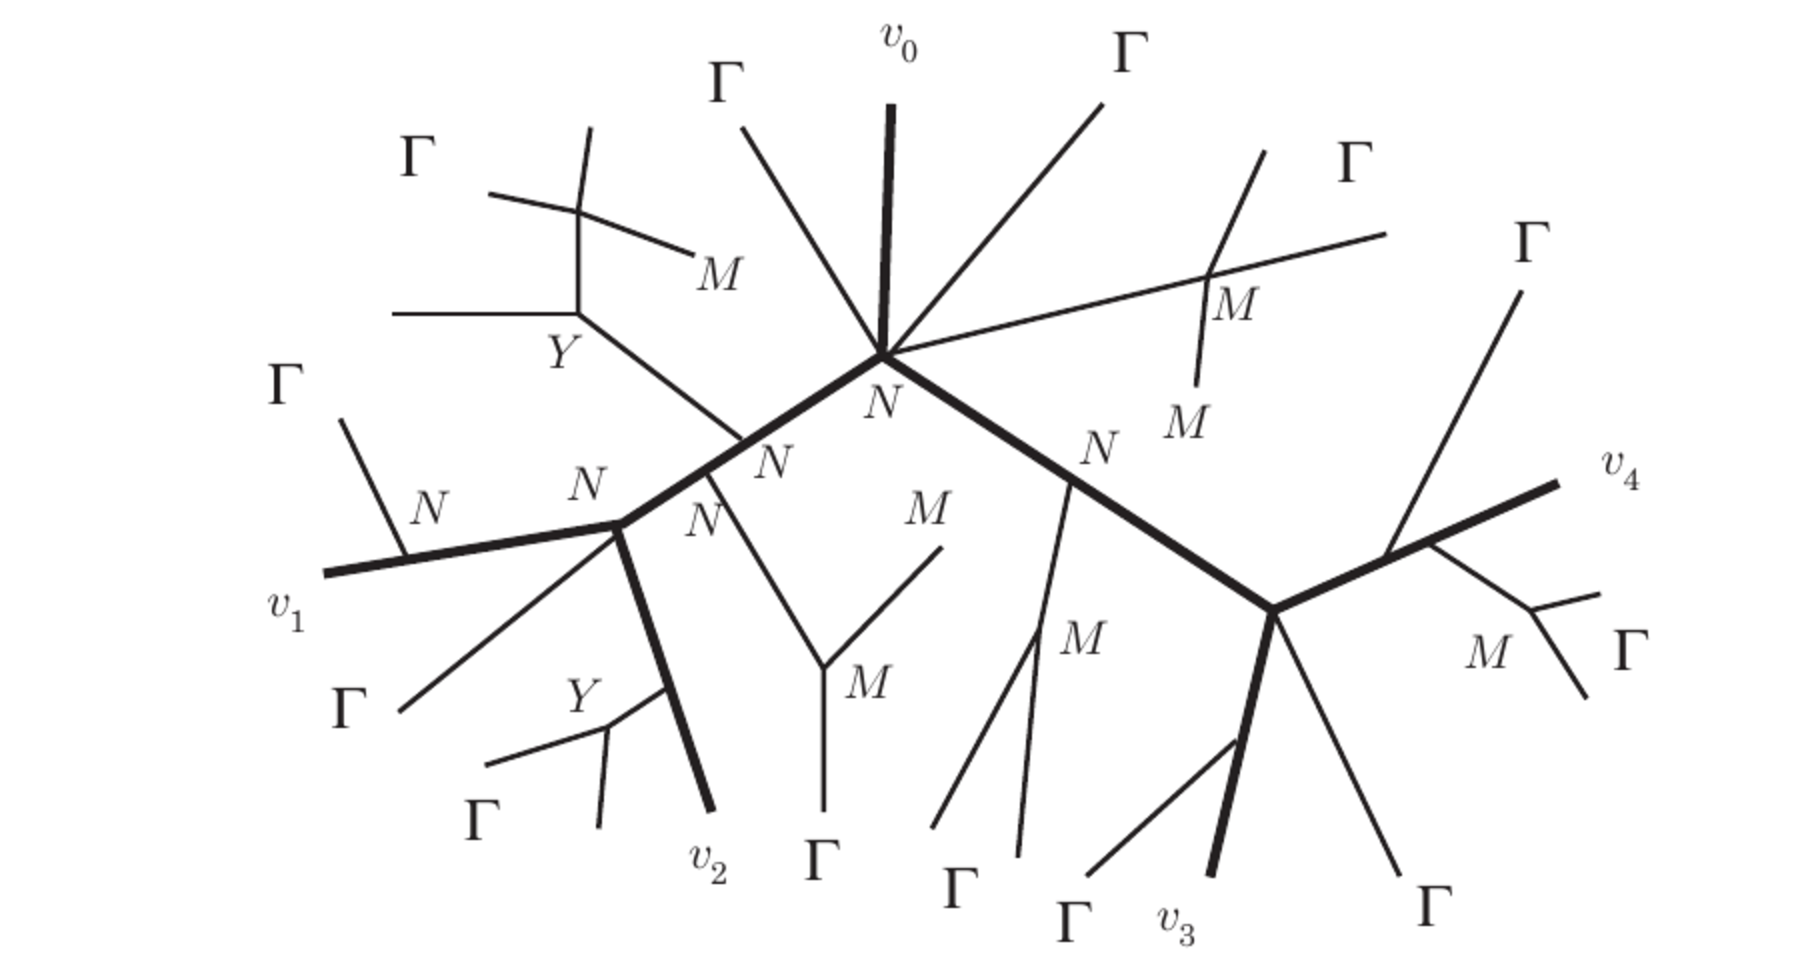
\includegraphics[width=.76\textwidth]{chapters/ch07-transversality/figures/phys-646-figure-7-4-18-clean-crop.png}
\par\smallskip
{\renewcommand{\thefigure}{7.4.18}\refstepcounter{figure}
\normalfont\bfseries 图~\thefigure\label{fig:7-4-18}}
\end{minipage}\par\medskip

把引理~\ref{lem:7-4-127}、
定理~\ref{thm:7-4-132}
与命题~\ref{prop:7-4-134}
推广到滤过 $A_\infty$ 双模语境的工作，
留给读者完成。
\end{remark}
